\documentclass[]{article}
\usepackage{lmodern}
\usepackage{amssymb,amsmath}
\usepackage{ifxetex,ifluatex}
\usepackage{fixltx2e} % provides \textsubscript
\ifnum 0\ifxetex 1\fi\ifluatex 1\fi=0 % if pdftex
  \usepackage[T1]{fontenc}
  \usepackage[utf8]{inputenc}
\else % if luatex or xelatex
  \ifxetex
    \usepackage{mathspec}
  \else
    \usepackage{fontspec}
  \fi
  \defaultfontfeatures{Ligatures=TeX,Scale=MatchLowercase}
\fi
% use upquote if available, for straight quotes in verbatim environments
\IfFileExists{upquote.sty}{\usepackage{upquote}}{}
% use microtype if available
\IfFileExists{microtype.sty}{%
\usepackage{microtype}
\UseMicrotypeSet[protrusion]{basicmath} % disable protrusion for tt fonts
}{}
\usepackage[margin=1in]{geometry}
\usepackage{hyperref}
\hypersetup{unicode=true,
            pdftitle={HW3},
            pdfauthor={Po-Sheng Lee},
            pdfborder={0 0 0},
            breaklinks=true}
\urlstyle{same}  % don't use monospace font for urls
\usepackage{graphicx,grffile}
\makeatletter
\def\maxwidth{\ifdim\Gin@nat@width>\linewidth\linewidth\else\Gin@nat@width\fi}
\def\maxheight{\ifdim\Gin@nat@height>\textheight\textheight\else\Gin@nat@height\fi}
\makeatother
% Scale images if necessary, so that they will not overflow the page
% margins by default, and it is still possible to overwrite the defaults
% using explicit options in \includegraphics[width, height, ...]{}
\setkeys{Gin}{width=\maxwidth,height=\maxheight,keepaspectratio}
\IfFileExists{parskip.sty}{%
\usepackage{parskip}
}{% else
\setlength{\parindent}{0pt}
\setlength{\parskip}{6pt plus 2pt minus 1pt}
}
\setlength{\emergencystretch}{3em}  % prevent overfull lines
\providecommand{\tightlist}{%
  \setlength{\itemsep}{0pt}\setlength{\parskip}{0pt}}
\setcounter{secnumdepth}{0}
% Redefines (sub)paragraphs to behave more like sections
\ifx\paragraph\undefined\else
\let\oldparagraph\paragraph
\renewcommand{\paragraph}[1]{\oldparagraph{#1}\mbox{}}
\fi
\ifx\subparagraph\undefined\else
\let\oldsubparagraph\subparagraph
\renewcommand{\subparagraph}[1]{\oldsubparagraph{#1}\mbox{}}
\fi

%%% Use protect on footnotes to avoid problems with footnotes in titles
\let\rmarkdownfootnote\footnote%
\def\footnote{\protect\rmarkdownfootnote}

%%% Change title format to be more compact
\usepackage{titling}

% Create subtitle command for use in maketitle
\newcommand{\subtitle}[1]{
  \posttitle{
    \begin{center}\large#1\end{center}
    }
}

\setlength{\droptitle}{-2em}

  \title{HW3}
    \pretitle{\vspace{\droptitle}\centering\huge}
  \posttitle{\par}
    \author{Po-Sheng Lee}
    \preauthor{\centering\large\emph}
  \postauthor{\par}
      \predate{\centering\large\emph}
  \postdate{\par}
    \date{2019/5/21}


\begin{document}
\maketitle

\section{Question 1}\label{question-1}

\begin{itemize}
\tightlist
\item
  Using the \texttt{VMAorder}, at order 2 we cannot reject the null
  hypothesis of zero correlation matrix. Thus the order should be set at
  1.
\end{itemize}

\begin{verbatim}
## Q(j,m) Statistics:  
##          j     Q(j,m)   p-value
##  [1,]   1.00    226.19     0.01
##  [2,]   2.00    164.05     0.63
##  [3,]   3.00    139.75     0.90
##  [4,]   4.00    127.43     0.93
##  [5,]   5.00    114.24     0.97
##  [6,]   6.00    102.07     0.98
##  [7,]   7.00     95.66     0.98
##  [8,]   8.00     91.13     0.96
##  [9,]   9.00     77.50     0.99
## [10,]  10.00     73.19     0.98
## [11,]  11.00     66.04     0.97
## [12,]  12.00     60.69     0.96
## [13,]  13.00     54.96     0.93
## [14,]  14.00     45.97     0.95
## [15,]  15.00     35.81     0.97
## [16,]  16.00     29.53     0.96
## [17,]  17.00     22.51     0.96
## [18,]  18.00     16.72     0.94
## [19,]  19.00      8.62     0.97
## [20,]  20.00      7.21     0.61
\end{verbatim}

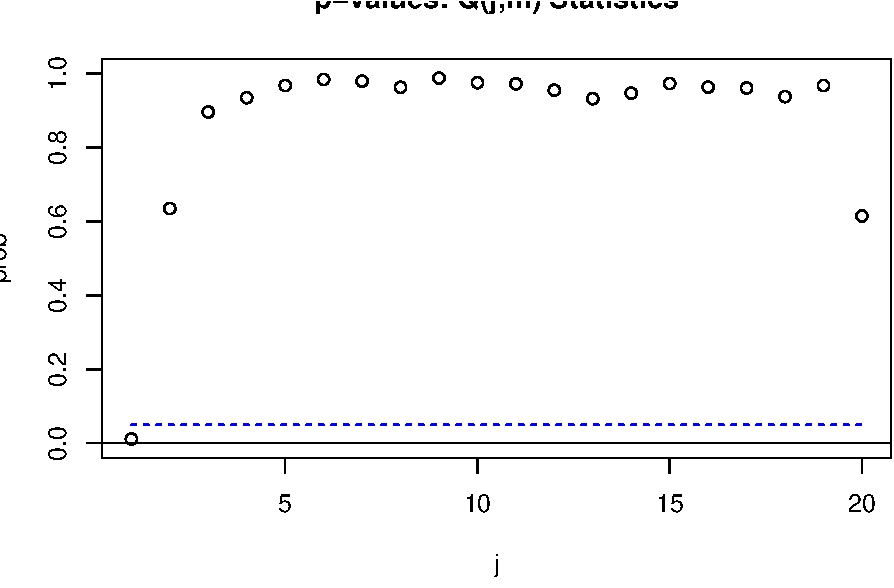
\includegraphics{HW3_files/figure-latex/unnamed-chunk-1-1.pdf}

\begin{itemize}
\tightlist
\item
  The estimated model via conditional likelihood is
  \(z_{t} = a_{t} - \left[\begin{array}{rrr}-0.31 & -0.04 & -0.33 \\-0.07 & -0.12 & -0.31 \\-0.25 & -0.15 & -0.47\end{array}\right]a_{t-1}\)
  where
  \(\sum_{a} = \left[\begin{array}{rrr}0.77 & 0.13 & 0.23 \\0.13 & 0.84 & 0.13 \\ 0.23 & 0.13 & 0.48\end{array}\right]\)
\end{itemize}

The refined model is not reported because the AIC and BIC is lower than
the original model.

\begin{verbatim}
## Number of parameters:  9 
## initial estimates:  -0.0908 0.0381 -0.242 0.0437 -0.0803 -0.2434 -0.2619 -0.1497 -0.4906 
## Par. Lower-bounds:  -0.3445 -0.1587 -0.5232 -0.192 -0.2631 -0.5046 -0.4722 -0.3128 -0.7236 
## Par. Upper-bounds:  0.163 0.2349 0.0392 0.2794 0.1026 0.0179 -0.0517 0.0133 -0.2576 
## Final   Estimates:  -0.3094283 -0.03978208 -0.3332371 -0.06886809 -0.1186957 -0.3117598 -0.2507167 -0.1452615 -0.4648592 
## 
## Coefficient(s):
##        Estimate  Std. Error  t value Pr(>|t|)    
##  [1,]  -0.30943     0.07012   -4.413 1.02e-05 ***
##  [2,]  -0.03978     0.06722   -0.592 0.553961    
##  [3,]  -0.33324     0.10015   -3.327 0.000877 ***
##  [4,]  -0.06887     0.09040   -0.762 0.446184    
##  [5,]  -0.11870     0.07113   -1.669 0.095152 .  
##  [6,]  -0.31176     0.11351   -2.746 0.006025 ** 
##  [7,]  -0.25072     0.05670   -4.422 9.78e-06 ***
##  [8,]  -0.14526     0.04774   -3.043 0.002344 ** 
##  [9,]  -0.46486     0.06402   -7.261 3.83e-13 ***
## ---
## Signif. codes:  0 '***' 0.001 '**' 0.01 '*' 0.05 '.' 0.1 ' ' 1
## --- 
## Estimates in matrix form: 
## MA coefficient matrix 
## MA( 1 )-matrix 
##         [,1]    [,2]   [,3]
## [1,] -0.3094 -0.0398 -0.333
## [2,] -0.0689 -0.1187 -0.312
## [3,] -0.2507 -0.1453 -0.465
##   
## Residuals cov-matrix: 
##           [,1]      [,2]      [,3]
## [1,] 0.7703965 0.1292742 0.2255974
## [2,] 0.1292742 0.8376136 0.1292353
## [3,] 0.2255974 0.1292353 0.4849380
## ---- 
## aic=  -1.241557 
## bic=  -1.063296
\end{verbatim}

\begin{verbatim}
## Number of parameters:  7 
## initial estimates:  0.3094 0.3332 0.1187 0.3118 0.2507 0.1453 0.4649 
## Par. Lower-bounds:  0.1692 0.1329 -0.0236 0.0847 0.1373 0.0498 0.3368 
## Par. Upper-bounds:  0.4497 0.5335 0.2609 0.5388 0.3641 0.2407 0.5929 
## Final   Estimates:  0.1691957 0.1329402 -0.02355494 0.08473165 0.1373234 0.04978338 0.3368244 
## 
## Coefficient(s):
##       Estimate  Std. Error  t value Pr(>|t|)    
## [1,]   0.16920     0.07596    2.227   0.0259 *  
## [2,]   0.13294     0.08520    1.560   0.1187    
## [3,]  -0.02355     0.08755   -0.269   0.7879    
## [4,]   0.08473     0.22843    0.371   0.7107    
## [5,]   0.13732     0.07034    1.952   0.0509 .  
## [6,]   0.04978     0.15430    0.323   0.7470    
## [7,]   0.33682     0.06145    5.481 4.22e-08 ***
## ---
## Signif. codes:  0 '***' 0.001 '**' 0.01 '*' 0.05 '.' 0.1 ' ' 1
## --- 
## Estimates in matrix form: 
## MA coefficient matrix 
## MA( 1 )-matrix 
##       [,1]    [,2]   [,3]
## [1,] 0.169  0.0000 0.1329
## [2,] 0.000 -0.0236 0.0847
## [3,] 0.137  0.0498 0.3368
##   
## Residuals cov-matrix: 
##           [,1]      [,2]      [,3]
## [1,] 1.9486657 0.6481247 1.7367433
## [2,] 0.6481247 1.0927888 0.8401055
## [3,] 1.7367433 0.8401055 2.4010122
## ---- 
## aic=  0.3722638 
## bic=  0.5109113
\end{verbatim}

\begin{itemize}
\tightlist
\item
  The estimated model via exact likelihood is
  \(z_{t} = a_{t} - \left[\begin{array}{rrr}-0.31 & -0.04 & -0.33 \\-0.07 & -0.12 & -0.32 \\-0.25 & -0.15 & -0.47\end{array}\right]a_{t-1}\)
\end{itemize}

where
\(\sum_{a} = \left[\begin{array}{rrr}0.77 & 0.13 & 0.23 \\0.13 & 0.84 & 0.13 \\ 0.23 & 0.13 & 0.48\end{array}\right]\)

The refined model is not reported because the AIC and BIC is about the
same as the original model.

\begin{itemize}
\tightlist
\item
  The conditional likelihood and exact likelihood yield similar model
  estimation. The only difference is the refined model in conditional
  likelihood method perform very bad.
\end{itemize}

\begin{verbatim}
## Number of parameters:  9 
## initial estimates:  -0.09077102 0.03809237 -0.2420405 0.04371478 -0.08025046 -0.2433616 -0.2619416 -0.1497472 -0.4906046 
## Par. Lower-bounds:  -0.3444992 -0.1586684 -0.5232392 -0.1920115 -0.2630512 -0.5046094 -0.4721731 -0.3127773 -0.7235973 
## Par. Upper-bounds:  0.1629571 0.2348532 0.03915819 0.279441 0.1025502 0.01788616 -0.05171013 0.01328282 -0.2576118 
## Final   Estimates:  -0.3087083 -0.03939251 -0.3299444 -0.07151888 -0.1217398 -0.3199985 -0.2508374 -0.1474073 -0.4665748 
## 
## Coefficient(s):
##        Estimate  Std. Error  t value Pr(>|t|)    
##  [1,]  -0.30871     0.06977   -4.425 9.65e-06 ***
##  [2,]  -0.03939     0.06718   -0.586 0.557641    
##  [3,]  -0.32994     0.10021   -3.293 0.000992 ***
##  [4,]  -0.07152     0.08991   -0.795 0.426327    
##  [5,]  -0.12174     0.07114   -1.711 0.087026 .  
##  [6,]  -0.32000     0.11344   -2.821 0.004791 ** 
##  [7,]  -0.25084     0.05627   -4.457 8.29e-06 ***
##  [8,]  -0.14741     0.04764   -3.094 0.001973 ** 
##  [9,]  -0.46657     0.06347   -7.352 1.96e-13 ***
## ---
## Signif. codes:  0 '***' 0.001 '**' 0.01 '*' 0.05 '.' 0.1 ' ' 1
## --- 
## Estimates in matrix form: 
## MA coefficient matrix 
## MA( 1 )-matrix 
##         [,1]    [,2]   [,3]
## [1,] -0.3087 -0.0394 -0.330
## [2,] -0.0715 -0.1217 -0.320
## [3,] -0.2508 -0.1474 -0.467
##   
## Residuals cov-matrix: 
##           [,1]      [,2]      [,3]
## [1,] 0.7713609 0.1284639 0.2260848
## [2,] 0.1284639 0.8364958 0.1282914
## [3,] 0.2260848 0.1282914 0.4849362
## ---- 
## aic=  -1.241433 
## bic=  -1.35908
\end{verbatim}

\begin{verbatim}
## Number of parameters:  7 
## initial estimates:  -0.3087083 -0.3299444 -0.1217398 -0.3199985 -0.2508374 -0.1474073 -0.4665748 
## Par. Lower-bounds:  -0.3784757 -0.4301507 -0.1928785 -0.4334417 -0.3071115 -0.1950452 -0.5300401 
## Par. Upper-bounds:  -0.2389409 -0.229738 -0.05060102 -0.2065552 -0.1945634 -0.0997694 -0.4031095 
## Final   Estimates:  -0.3128601 -0.3367432 -0.1298341 -0.3565174 -0.2482166 -0.1483992 -0.4634174 
## 
## Coefficient(s):
##       Estimate  Std. Error  t value Pr(>|t|)    
## [1,]  -0.31286     0.06930   -4.515 6.34e-06 ***
## [2,]  -0.33674     0.10110   -3.331 0.000866 ***
## [3,]  -0.12983     0.07021   -1.849 0.064427 .  
## [4,]  -0.35652     0.10972   -3.249 0.001156 ** 
## [5,]  -0.24822     0.05595   -4.436 9.16e-06 ***
## [6,]  -0.14840     0.04713   -3.148 0.001642 ** 
## [7,]  -0.46342     0.06273   -7.387 1.50e-13 ***
## ---
## Signif. codes:  0 '***' 0.001 '**' 0.01 '*' 0.05 '.' 0.1 ' ' 1
## --- 
## Estimates in matrix form: 
## MA coefficient matrix 
## MA( 1 )-matrix 
##        [,1]   [,2]   [,3]
## [1,] -0.313  0.000 -0.337
## [2,]  0.000 -0.130 -0.357
## [3,] -0.248 -0.148 -0.463
##   
## Residuals cov-matrix: 
##           [,1]      [,2]      [,3]
## [1,] 0.7741764 0.1325708 0.2254809
## [2,] 0.1325708 0.8455543 0.1312927
## [3,] 0.2254809 0.1312927 0.4824201
## ---- 
## aic=  -1.260071 
## bic=  -1.351574
\end{verbatim}

\section{Question 2}\label{question-2}

\begin{itemize}
\tightlist
\item
  The \texttt{VARorder} shows the best order to be selected is order 1
  according to every criteria.
\end{itemize}

\begin{verbatim}
## selected order: aic =  1 
## selected order: bic =  1 
## selected order: hq =  1 
## Summary table:  
##        p     AIC     BIC      HQ    M(p) p-value
##  [1,]  0 -1.8572 -1.8572 -1.8572  0.0000  0.0000
##  [2,]  1 -2.2200 -2.0418 -2.1476 65.1040  0.0000
##  [3,]  2 -2.1354 -1.7789 -1.9906  4.3823  0.8845
##  [4,]  3 -2.0979 -1.5631 -1.8806 10.3679  0.3215
##  [5,]  4 -2.1356 -1.4225 -1.8459 19.6547  0.0202
##  [6,]  5 -2.1089 -1.2176 -1.7468 11.2328  0.2601
##  [7,]  6 -2.0288 -0.9593 -1.5944  4.5320  0.8731
##  [8,]  7 -1.9409 -0.6930 -1.4340  3.4844  0.9420
##  [9,]  8 -1.9792 -0.5531 -1.3999 17.8648  0.0368
## [10,]  9 -1.8997 -0.2954 -1.2480  4.2528  0.8940
## [11,] 10 -1.8322 -0.0496 -1.1081  5.4369  0.7947
## [12,] 11 -1.7532  0.2077 -0.9567  4.0787  0.9062
## [13,] 12 -1.6988  0.4403 -0.8299  6.4865  0.6904
## [14,] 13 -1.6728  0.6446 -0.7314  9.1102  0.4272
\end{verbatim}

\begin{itemize}
\tightlist
\item
  The refined VAR(1) model can be written as
  \(z_{t} = \left[\begin{array}{ccc}0.5 \\ 0.28 \\ 0.1\end{array}\right] + \left[\begin{array}{rrr}0.137 & 0 & 0.29 \\0 & 0.08 & 0.23 \\0.25 & 0.13 & 0.41\end{array}\right]z_{t-1} + a_{t}\)
\end{itemize}

where
\(\sum_{a} = \left[\begin{array}{rrr}0.08 & 0 & 0.08\\0 & 0.081 & 0.1 \\ 0.07 & 0.06 & 0.07\end{array}\right]\)

\begin{itemize}
\tightlist
\item
  Based on the AIC and BIC, VAR(1) model seems to perform better than
  VMA(1) model.
\end{itemize}

\begin{verbatim}
## Constant term: 
## Estimates:  0.5033322 0.2823586 0.1028284 
## Std.Error:  0.08886738 0.1143083 0.08032438 
## AR coefficient matrix 
## AR( 1 )-matrix 
##         [,1]    [,2]  [,3]
## [1,]  0.1356 -0.0215 0.295
## [2,] -0.0427  0.0807 0.238
## [3,]  0.2462  0.1295 0.411
## standard error 
##        [,1]   [,2]   [,3]
## [1,] 0.0797 0.0633 0.0788
## [2,] 0.1025 0.0814 0.1014
## [3,] 0.0721 0.0572 0.0713
##   
## Residuals cov-mtx: 
##             [,1]        [,2]       [,3]
## [1,]  0.46022141 -0.03064453 0.04282989
## [2,] -0.03064453  0.76144307 0.04602688
## [3,]  0.04282989  0.04602688 0.37599047
##   
## det(SSE) =  0.1289136 
## AIC =  -1.930966 
## BIC =  -1.752705 
## HQ  =  -1.858553
\end{verbatim}

\begin{verbatim}
## Constant term: 
## Estimates:  0.4961847 0.2558718 0.1028284 
## Std.Error:  0.08608764 0.0946918 0.08032438 
## AR coefficient matrix 
## AR( 1 )-matrix 
##       [,1]  [,2]  [,3]
## [1,] 0.137 0.000 0.291
## [2,] 0.000 0.082 0.226
## [3,] 0.246 0.130 0.411
## standard error 
##        [,1]   [,2]   [,3]
## [1,] 0.0794 0.0000 0.0773
## [2,] 0.0000 0.0812 0.0972
## [3,] 0.0721 0.0572 0.0713
##   
## Residuals cov-mtx: 
##             [,1]        [,2]       [,3]
## [1,]  0.46058076 -0.03062391 0.04282989
## [2,] -0.03062391  0.76233432 0.04602688
## [3,]  0.04282989  0.04602688 0.37599047
##   
## det(SSE) =  0.129169 
## AIC =  -1.955131 
## BIC =  -1.816483 
## HQ  =  -1.89881
\end{verbatim}

\section{Question 3}\label{question-3}

The VAR(1) model can be written as
\(z_{t} = \left[\begin{array}{ccc}0.27 \\ 0.21 \\ 0.08\end{array}\right] + \left[\begin{array}{rrr}0.137 & 0 & 0.29 \\0 & 0.08 & 0.23 \\0.25 & 0.13 & 0.41\end{array}\right]z_{t-1} + a_{t}\)

where
\(\sum_{a} = \left[\begin{array}{rrr}0.36 & 0.07 & 0.13\\0.07 & 0.33 & 0.02 \\ 0.13 & 0.02 & 0.32\end{array}\right]\)

The model checking shows that it is a good model specification.

\begin{verbatim}
## selected order: aic =  1 
## selected order: bic =  1 
## selected order: hq =  1 
## Summary table:  
##        p     AIC     BIC      HQ     M(p) p-value
##  [1,]  0 -3.3030 -3.3030 -3.3030   0.0000  0.0000
##  [2,]  1 -4.1235 -3.9452 -4.0511 127.1173  0.0000
##  [3,]  2 -4.0932 -3.7367 -3.9484  11.5761  0.2383
##  [4,]  3 -4.0188 -3.4840 -3.8016   5.5989  0.7793
##  [5,]  4 -4.0287 -3.3157 -3.7390  16.1339  0.0641
##  [6,]  5 -3.9495 -3.0582 -3.5874   4.7473  0.8558
##  [7,]  6 -3.9221 -2.8525 -3.4876  10.8705  0.2847
##  [8,]  7 -3.8428 -2.5949 -3.3359   4.5071  0.8750
##  [9,]  8 -3.8743 -2.4483 -3.2950  17.0859  0.0474
## [10,]  9 -3.8537 -2.2494 -3.2020  10.8198  0.2883
## [11,] 10 -3.7811 -1.9985 -3.0569   4.8798  0.8447
## [12,] 11 -3.7917 -1.8308 -2.9952  13.5361  0.1398
## [13,] 12 -3.8879 -1.7488 -3.0189  21.9172  0.0091
## [14,] 13 -3.8384 -1.5210 -2.8970   6.7767  0.6604
\end{verbatim}

\begin{verbatim}
## Constant term: 
## Estimates:  0.2670306 0.2056176 0.08174096 
## Std.Error:  0.07089002 0.06781075 0.06737615 
## AR coefficient matrix 
## AR( 1 )-matrix 
##        [,1]  [,2]   [,3]
## [1,] 0.1350 0.386 0.1532
## [2,] 0.0885 0.464 0.0539
## [3,] 0.3469 0.285 0.2216
## standard error 
##        [,1]   [,2]   [,3]
## [1,] 0.0896 0.0791 0.0816
## [2,] 0.0857 0.0756 0.0781
## [3,] 0.0852 0.0752 0.0776
##   
## Residuals cov-mtx: 
##            [,1]       [,2]      [,3]
## [1,] 0.35502986 0.06843442 0.1335999
## [2,] 0.06843442 0.32485670 0.0172737
## [3,] 0.13359986 0.01727370 0.3207059
##   
## det(SSE) =  0.02989788 
## AIC =  -3.392321 
## BIC =  -3.21406 
## HQ  =  -3.319908
\end{verbatim}

\begin{verbatim}
## Constant term: 
## Estimates:  0.2670306 0.2143776 0.08174096 
## Std.Error:  0.07089002 0.0664984 0.06737615 
## AR coefficient matrix 
## AR( 1 )-matrix 
##       [,1]  [,2]  [,3]
## [1,] 0.135 0.386 0.153
## [2,] 0.120 0.469 0.000
## [3,] 0.347 0.285 0.222
## standard error 
##        [,1]   [,2]   [,3]
## [1,] 0.0896 0.0791 0.0816
## [2,] 0.0729 0.0750 0.0000
## [3,] 0.0852 0.0752 0.0776
##   
## Residuals cov-mtx: 
##            [,1]       [,2]      [,3]
## [1,] 0.35502986 0.06843442 0.1335999
## [2,] 0.06843442 0.32590484 0.0172737
## [3,] 0.13359986 0.01727370 0.3207059
##   
## det(SSE) =  0.02999851 
## AIC =  -3.402032 
## BIC =  -3.243578 
## HQ  =  -3.337666
\end{verbatim}

\begin{verbatim}
## [1] "Covariance matrix:"
##        US     UK     CA
## US 0.3574 0.0689 0.1345
## UK 0.0689 0.3281 0.0174
## CA 0.1345 0.0174 0.3228
## CCM at lag:  0 
##       [,1]   [,2]   [,3]
## [1,] 1.000 0.2012 0.3959
## [2,] 0.201 1.0000 0.0534
## [3,] 0.396 0.0534 1.0000
## Simplified matrix: 
## CCM at lag:  1 
## . . . 
## . . . 
## . . . 
## CCM at lag:  2 
## . . . 
## . . . 
## . . . 
## CCM at lag:  3 
## . . . 
## + . . 
## . . . 
## CCM at lag:  4 
## . . - 
## . . . 
## . . . 
## CCM at lag:  5 
## . . . 
## . . . 
## . . . 
## CCM at lag:  6 
## . . - 
## . . . 
## . . . 
## CCM at lag:  7 
## . . . 
## . . . 
## . . . 
## CCM at lag:  8 
## . . . 
## . . . 
## . . . 
## CCM at lag:  9 
## . . . 
## . . . 
## . . . 
## CCM at lag:  10 
## . + . 
## . . . 
## . . . 
## CCM at lag:  11 
## . . . 
## . . . 
## - . . 
## CCM at lag:  12 
## . - . 
## . . . 
## . - . 
## CCM at lag:  13 
## . . . 
## . . . 
## . . . 
## CCM at lag:  14 
## . . . 
## . . . 
## . . . 
## CCM at lag:  15 
## . . . 
## . . . 
## . - . 
## CCM at lag:  16 
## . . . 
## . . . 
## . . . 
## CCM at lag:  17 
## . . . 
## . . . 
## . . . 
## CCM at lag:  18 
## . . . 
## . . . 
## - . . 
## CCM at lag:  19 
## . . . 
## . . . 
## + . . 
## CCM at lag:  20 
## . . . 
## . . . 
## . . . 
## CCM at lag:  21 
## . . . 
## . . . 
## . . . 
## CCM at lag:  22 
## . . . 
## . . . 
## . . . 
## CCM at lag:  23 
## . . . 
## . . . 
## . . . 
## CCM at lag:  24 
## . . . 
## . . . 
## . + .
\end{verbatim}

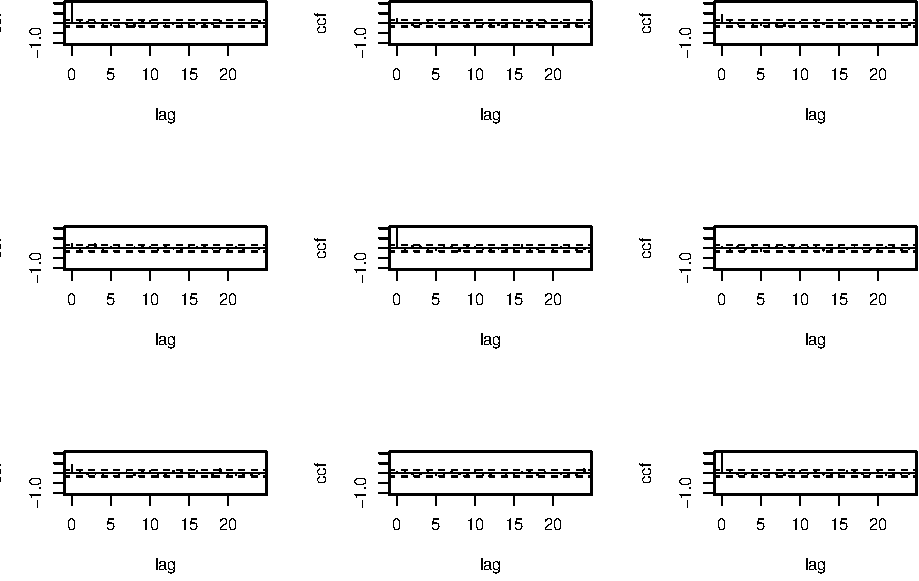
\includegraphics{HW3_files/figure-latex/unnamed-chunk-6-1.pdf}

\begin{verbatim}
## Hit Enter for p-value plot of individual ccm:
\end{verbatim}

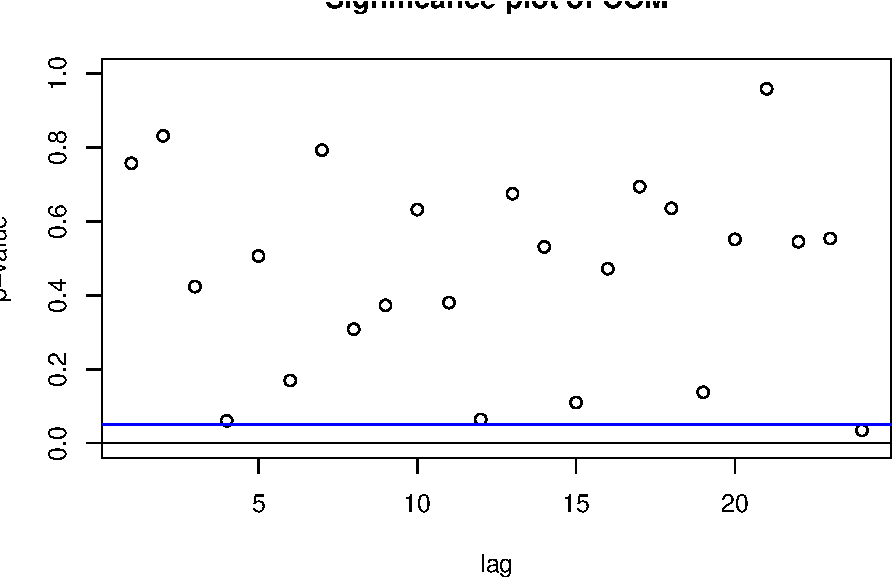
\includegraphics{HW3_files/figure-latex/unnamed-chunk-6-2.pdf}

\begin{verbatim}
## Hit Enter to compute MQ-statistics: 
## 
## Ljung-Box Statistics:  
##         m       Q(m)     df    p-value
##  [1,]   1.0       5.9     9.0     0.75
##  [2,]   2.0      11.0    18.0     0.89
##  [3,]   3.0      20.3    27.0     0.82
##  [4,]   4.0      36.8    36.0     0.43
##  [5,]   5.0      45.2    45.0     0.46
##  [6,]   6.0      58.2    54.0     0.32
##  [7,]   7.0      63.8    63.0     0.45
##  [8,]   8.0      74.5    72.0     0.40
##  [9,]   9.0      84.3    81.0     0.38
## [10,]  10.0      91.4    90.0     0.44
## [11,]  11.0     101.2    99.0     0.42
## [12,]  12.0     117.6   108.0     0.25
## [13,]  13.0     124.3   117.0     0.30
## [14,]  14.0     132.4   126.0     0.33
## [15,]  15.0     147.0   135.0     0.23
## [16,]  16.0     155.8   144.0     0.24
## [17,]  17.0     162.3   153.0     0.29
## [18,]  18.0     169.4   162.0     0.33
## [19,]  19.0     183.2   171.0     0.25
## [20,]  20.0     191.1   180.0     0.27
## [21,]  21.0     194.3   189.0     0.38
## [22,]  22.0     202.3   198.0     0.40
## [23,]  23.0     210.2   207.0     0.42
## [24,]  24.0     228.5   216.0     0.27
\end{verbatim}

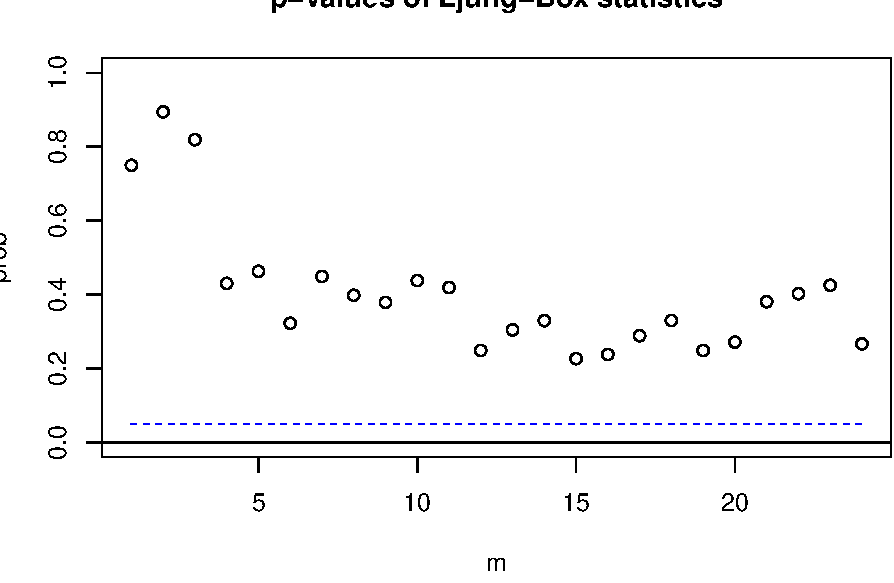
\includegraphics{HW3_files/figure-latex/unnamed-chunk-6-3.pdf}

\begin{verbatim}
## Hit Enter to obtain residual plots:
\end{verbatim}

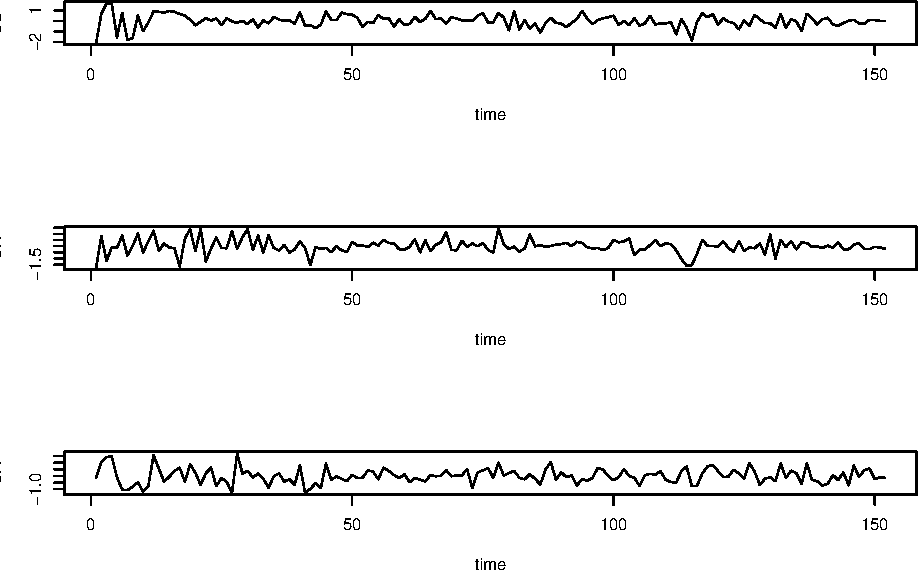
\includegraphics{HW3_files/figure-latex/unnamed-chunk-6-4.pdf}

\begin{itemize}
\tightlist
\item
  The impulse response function is shown in the following figures
\end{itemize}

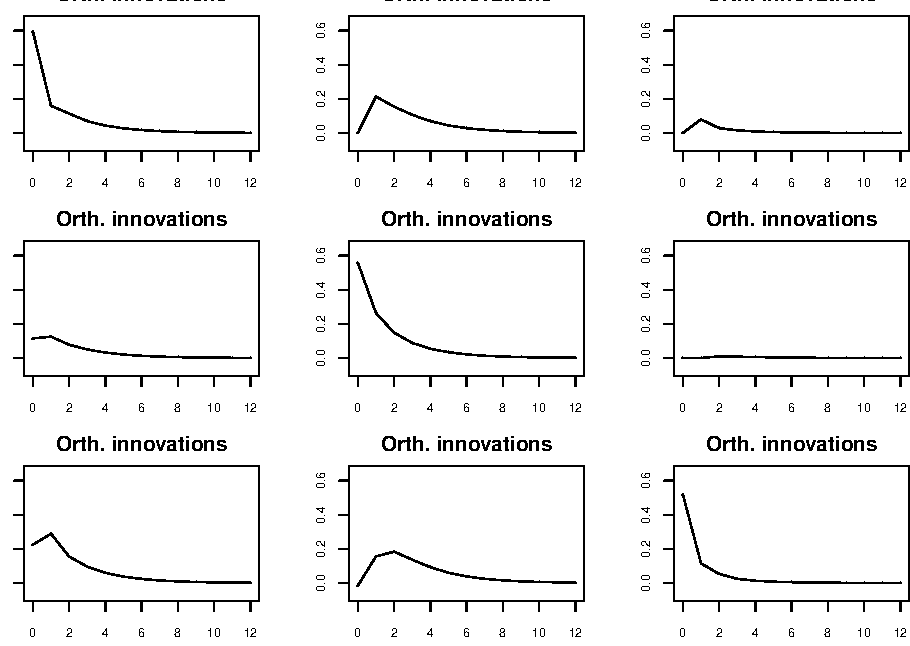
\includegraphics{HW3_files/figure-latex/unnamed-chunk-7-1.pdf}

\begin{verbatim}
## Press return to continue
\end{verbatim}

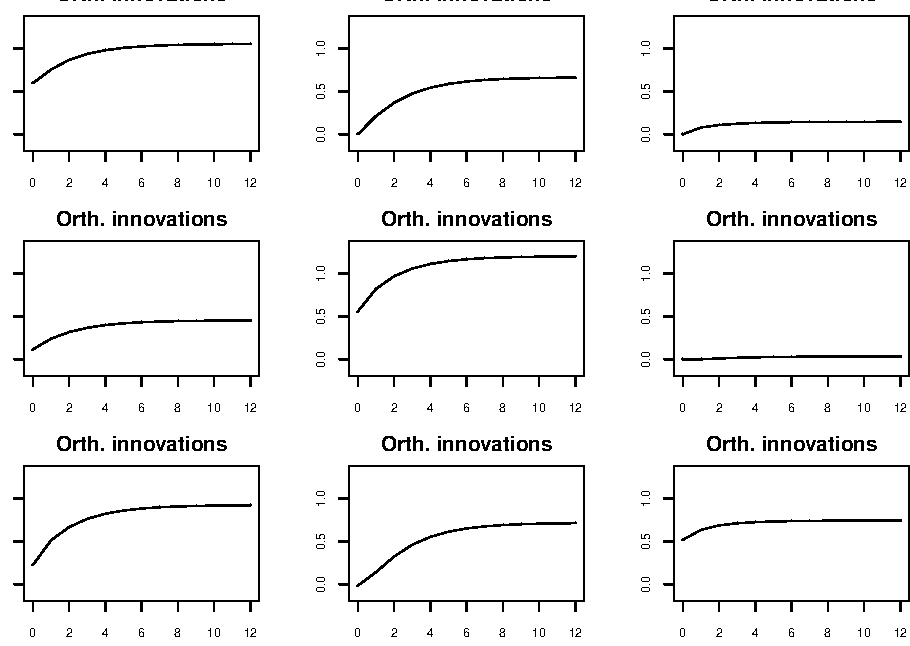
\includegraphics{HW3_files/figure-latex/unnamed-chunk-7-2.pdf}

\begin{itemize}
\tightlist
\item
  Using the t-test of MQ, the order should be set at 3. The VMA(3) model
  can be written as
  \(z_{t} = a_{t} - \left[\begin{array}{ccc}-0.28 & -0.54 & -0.11 \\ -0.16 & -0.4 & 0.28 \\ -0.5 & -0.51 & -0.31\end{array}\right]a_{t-1} - \left[\begin{array}{rrr}-0.096 & -0.29 & 0.16 \\-0.2 & -0.55 & 0.06 \\-0.22 & -0.16 & -0.13\end{array}\right]a_{t-2} - \left[\begin{array}{rrr}-0.216 & -0.02 & -0.2 \\-0.43 & -0.36 & -0.06 \\-0.19 & -0.007 & -0.17\end{array}\right]a_{t-3}\)
\end{itemize}

where
\(\sum_{a} = \left[\begin{array}{rrr}0.87 & 0.37 & 0.59\\0.37 & 0.65 & 0.17 \\ 0.59 & 0.17 & 0.9\end{array}\right]\)

-The model checking shows that MA representation is not a good model.
The \(\Psi\) of impulse response function is equal to the coefficeint of
MA model with a negative sign (\(-\theta\))

-The most significant difference of impulse response function is that AR
representation can estimate a impulse response coefficient with a longer
time lag while the MA representation itself is an impulse response
function. As a result, impulse response function of MA in this case is
not able to account for impulse with longer lag.

\begin{verbatim}
## Q(j,m) Statistics:  
##          j     Q(j,m)   p-value
##  [1,]   1.00    322.69     0.00
##  [2,]   2.00    230.66     0.00
##  [3,]   3.00    193.81     0.04
##  [4,]   4.00    174.59     0.11
##  [5,]   5.00    158.72     0.19
##  [6,]   6.00    150.62     0.17
##  [7,]   7.00    138.67     0.21
##  [8,]   8.00    123.57     0.32
##  [9,]   9.00    110.43     0.42
## [10,]  10.00    105.22     0.32
## [11,]  11.00    100.68     0.21
## [12,]  12.00     95.37     0.13
## [13,]  13.00     78.63     0.28
## [14,]  14.00     67.61     0.32
## [15,]  15.00     56.43     0.38
## [16,]  16.00     38.99     0.72
## [17,]  17.00     33.08     0.61
## [18,]  18.00     27.40     0.44
## [19,]  19.00     18.83     0.40
## [20,]  20.00      5.18     0.82
\end{verbatim}

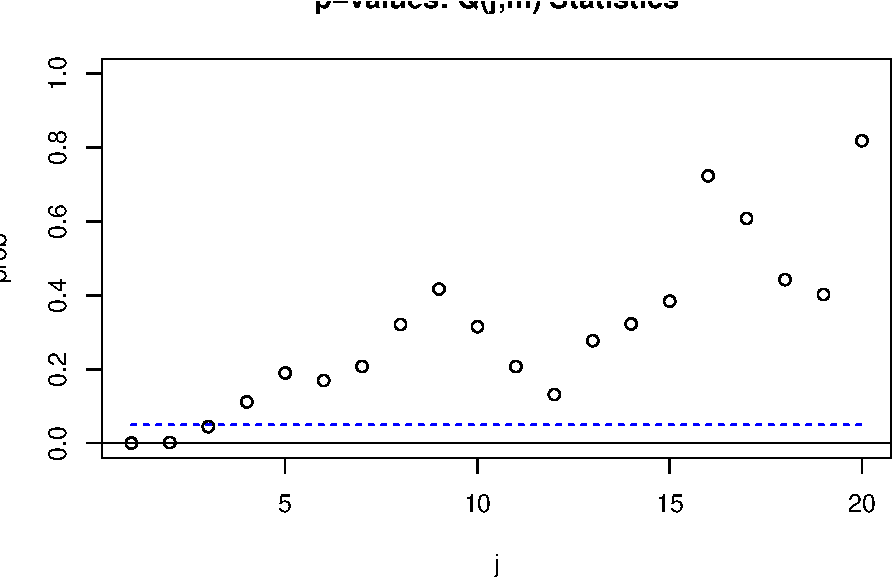
\includegraphics{HW3_files/figure-latex/unnamed-chunk-8-1.pdf}

\begin{verbatim}
## Number of parameters:  27 
## initial estimates:  -0.2023816 -0.4249283 -0.1129188 -0.2609783 -0.2849037 0.01740935 -0.09714983 -0.157729 -0.04368183 -0.08501424 -0.4300176 0.02284808 -0.0146786 -0.3877751 -0.1090357 -0.2737368 -0.1959458 0.10976 -0.4397776 -0.4142024 -0.2062877 -0.1950684 -0.4039806 -0.04474959 -0.09229529 -0.2076644 -0.05761171 
## Par. Lower-bounds:  -0.407275 -0.6214217 -0.3202763 -0.4649722 -0.4808613 -0.187883 -0.2936229 -0.3495268 -0.247319 -0.2684913 -0.6059727 -0.1628355 -0.1973501 -0.5632503 -0.29287 -0.4496736 -0.3676961 -0.07259216 -0.63094 -0.5975277 -0.399749 -0.3853915 -0.586806 -0.2362842 -0.2756016 -0.3866088 -0.247602 
## Par. Upper-bounds:  0.00251184 -0.2284349 0.09443871 -0.05698448 -0.08894608 0.2227017 0.09932319 0.03406878 0.1599553 0.09846282 -0.2540625 0.2085317 0.1679929 -0.2122998 0.07479861 -0.09779993 -0.02419558 0.2921121 -0.2486152 -0.2308771 -0.01282636 -0.004745307 -0.2211552 0.146785 0.091011 -0.02872006 0.1323786 
## Final   Estimates:  -0.2829096 -0.5400792 -0.110988 -0.09569793 -0.2879647 0.1631056 -0.215794 -0.01648834 -0.2028233 -0.1614176 -0.3986051 0.2273341 -0.2047771 -0.549056 0.06108905 -0.4317697 -0.3603384 -0.06235632 -0.501743 -0.5135271 -0.309257 -0.2191025 -0.1613954 -0.1333701 -0.1876784 -0.006715674 -0.1683318 
## 
## Coefficient(s):
##         Estimate  Std. Error  t value Pr(>|t|)    
##  [1,] -2.829e-01   3.412e-06   -82917   <2e-16 ***
##  [2,] -5.401e-01   6.514e-06   -82908   <2e-16 ***
##  [3,] -1.110e-01   1.339e-06   -82916   <2e-16 ***
##  [4,] -9.570e-02   1.154e-06   -82915   <2e-16 ***
##  [5,] -2.880e-01   3.473e-06   -82919   <2e-16 ***
##  [6,]  1.631e-01   1.967e-06    82912   <2e-16 ***
##  [7,] -2.158e-01   2.602e-06   -82919   <2e-16 ***
##  [8,] -1.649e-02   1.989e-07   -82916   <2e-16 ***
##  [9,] -2.028e-01   2.446e-06   -82919   <2e-16 ***
## [10,] -1.614e-01   1.947e-06   -82918   <2e-16 ***
## [11,] -3.986e-01   4.807e-06   -82925   <2e-16 ***
## [12,]  2.273e-01   2.742e-06    82918   <2e-16 ***
## [13,] -2.048e-01   2.470e-06   -82917   <2e-16 ***
## [14,] -5.491e-01   6.621e-06   -82928   <2e-16 ***
## [15,]  6.109e-02   7.367e-07    82917   <2e-16 ***
## [16,] -4.318e-01   5.207e-06   -82924   <2e-16 ***
## [17,] -3.603e-01   4.345e-06   -82924   <2e-16 ***
## [18,] -6.236e-02   7.520e-07   -82917   <2e-16 ***
## [19,] -5.017e-01   6.051e-06   -82918   <2e-16 ***
## [20,] -5.135e-01   6.193e-06   -82925   <2e-16 ***
## [21,] -3.093e-01   3.730e-06   -82917   <2e-16 ***
## [22,] -2.191e-01   2.642e-06   -82918   <2e-16 ***
## [23,] -1.614e-01   1.946e-06   -82918   <2e-16 ***
## [24,] -1.334e-01   1.608e-06   -82917   <2e-16 ***
## [25,] -1.877e-01   2.263e-06   -82917   <2e-16 ***
## [26,] -6.716e-03   8.099e-08   -82916   <2e-16 ***
## [27,] -1.683e-01   2.030e-06   -82917   <2e-16 ***
## ---
## Signif. codes:  0 '***' 0.001 '**' 0.01 '*' 0.05 '.' 0.1 ' ' 1
## --- 
## Estimates in matrix form: 
## MA coefficient matrix 
## MA( 1 )-matrix 
##        [,1]   [,2]   [,3]
## [1,] -0.283 -0.540 -0.111
## [2,] -0.161 -0.399  0.227
## [3,] -0.502 -0.514 -0.309
## MA( 2 )-matrix 
##         [,1]   [,2]    [,3]
## [1,] -0.0957 -0.288  0.1631
## [2,] -0.2048 -0.549  0.0611
## [3,] -0.2191 -0.161 -0.1334
## MA( 3 )-matrix 
##        [,1]     [,2]    [,3]
## [1,] -0.216 -0.01649 -0.2028
## [2,] -0.432 -0.36034 -0.0624
## [3,] -0.188 -0.00672 -0.1683
##   
## Residuals cov-matrix: 
##           [,1]      [,2]      [,3]
## [1,] 0.8695451 0.3650364 0.5929707
## [2,] 0.3650364 0.6531074 0.1665524
## [3,] 0.5929707 0.1665524 0.9002276
## ---- 
## aic=  -1.20948 
## bic=  -1.562421
\end{verbatim}

\section{Question 4}\label{question-4}

\begin{itemize}
\item
  The eigen values can be calculated from the square of deviation. The
  three largest are 1.34, 0.72 and 0.39. The first component can account
  for 44\% of the variations, and the first three component can account
  for 80\% of all the variations.
\item
  The first component get a taste of every country, the second component
  is comprised by three non-European countries minus two European
  countries and the third component is constituted by two North America
  countries minus other non North America countries.
\end{itemize}

\begin{verbatim}
##    Comp.1    Comp.2    Comp.3    Comp.4    Comp.5    Comp.6 
## 1.3405953 0.7229616 0.3886950 0.3131221 0.1916094 0.1114350
\end{verbatim}

\begin{verbatim}
## Importance of components:
##                           Comp.1    Comp.2    Comp.3    Comp.4     Comp.5
## Standard deviation     1.1578408 0.8502715 0.6234541 0.5595731 0.43773213
## Proportion of Variance 0.4369011 0.2356138 0.1266760 0.1020467 0.06244566
## Cumulative Proportion  0.4369011 0.6725148 0.7991909 0.9012376 0.96368325
##                            Comp.6
## Standard deviation     0.33381878
## Proportion of Variance 0.03631675
## Cumulative Proportion  1.00000000
\end{verbatim}

\begin{verbatim}
## 
## Loadings:
##    Comp.1 Comp.2 Comp.3 Comp.4 Comp.5 Comp.6
## US  0.484  0.248  0.154  0.145  0.811       
## UK  0.400        -0.246 -0.851        -0.220
## FR  0.266 -0.146        -0.118 -0.123  0.937
## AU  0.309  0.467 -0.677  0.394 -0.270       
## GE  0.485 -0.783 -0.132  0.272        -0.235
## CA  0.451  0.285  0.664  0.105 -0.497 -0.129
## 
##                Comp.1 Comp.2 Comp.3 Comp.4 Comp.5 Comp.6
## SS loadings     1.000  1.000  1.000  1.000  1.000  1.000
## Proportion Var  0.167  0.167  0.167  0.167  0.167  0.167
## Cumulative Var  0.167  0.333  0.500  0.667  0.833  1.000
\end{verbatim}

\section{Question 5}\label{question-5}

\begin{itemize}
\tightlist
\item
  The VAR(1) for the growth rate series can be written as
\end{itemize}

\(z_{t} = \left[\begin{array}{cccccc}0.31\\0.27\\ 0.13\\0.54\\0.12\\0 \end{array}\right] + \left[\begin{array}{rrrrrr}0.15 & 0.43 & -0.20 & 0 & 0 & 0.17 \\0.17 & 0.49 & 0 & -0.13 & 0 & 0 \\0.09 & 0.16 & 0.44 & 0 & -0.05 & 0 \\ 0 & 0.2 & -0.31 & 0.11 & 0 & 0.31\\ 0.24 & 0 & 0.69 & -0.15 & -0.13 & 0 \\ 0.32 & 0.31 & -0.21 & 0.13 & 0.09 & 0.25\end{array}\right]z_{t-1} + a_{t}\)

where
\(\sum_{a} = \left[\begin{array}{rrrrrr}0.35 & 0.066 & 0.046 & 0.12 & 0.089 & 0.13\\0.066 & 0.32 & 0.069 & 0.075 & 0.084 & 0.024 \\ 0.046 & 0.069 & 0.13 & 0.021 & 0.13 & 0.025 \\ 0.12 & 0.075 & 0.021 & 0.44 & -0.017 & 0.015 \\ 0.090 & 0.084 & 0.13 & -0.017 & 0.68 & 0.019 \\ 0.13 & 0.024 & 0.015 & 0.015 & 0.019 & 0.31 \end{array}\right]\)

\begin{verbatim}
## selected order: aic =  13 
## selected order: bic =  1 
## selected order: hq =  1 
## Summary table:  
##        p     AIC     BIC      HQ     M(p) p-value
##  [1,]  0 -6.8887 -6.8887 -6.8887   0.0000  0.0000
##  [2,]  1 -7.7959 -7.0829 -7.5063 182.5630  0.0000
##  [3,]  2 -7.7156 -6.2895 -7.1362  49.3614  0.0681
##  [4,]  3 -7.5512 -5.4121 -6.6823  36.9038  0.4269
##  [5,]  4 -7.5679 -4.7157 -6.4093  55.7927  0.0187
##  [6,]  5 -7.4977 -3.9324 -6.0494  43.4377  0.1841
##  [7,]  6 -7.3380 -3.0598 -5.6001  31.8750  0.6652
##  [8,]  7 -7.1339 -2.1425 -5.1063  25.7069  0.8983
##  [9,]  8 -7.3742 -1.6699 -5.0570  64.3401  0.0025
## [10,]  9 -7.5061 -1.0887 -4.8993  50.9105  0.0509
## [11,] 10 -7.4301 -0.2997 -4.5336  30.9780  0.7062
## [12,] 11 -7.6115  0.2320 -4.4253  47.2625  0.0991
## [13,] 12 -7.8454  0.7112 -4.3696  46.8496  0.1064
## [14,] 13 -8.1084  1.1612 -4.3429  44.3816  0.1593
\end{verbatim}

\begin{verbatim}
## Constant term: 
## Estimates:  0.3163104 0.2756356 0.1320467 0.5399103 0.1174305 0.07357535 
## Std.Error:  0.08301148 0.07903544 0.05114018 0.09316432 0.1156071 0.07812133 
## AR coefficient matrix 
## AR( 1 )-matrix 
##        [,1]  [,2]     [,3]    [,4]    [,5]   [,6]
## [1,] 0.1641 0.437 -0.17598 -0.0212 -0.0245 0.1708
## [2,] 0.1517 0.497 -0.00266 -0.1428 -0.0455 0.0564
## [3,] 0.0764 0.160  0.42812 -0.0230 -0.0513 0.0384
## [4,] 0.0369 0.189 -0.34466  0.1027  0.0278 0.2910
## [5,] 0.2095 0.083  0.63957 -0.1587 -0.1284 0.0287
## [6,] 0.3096 0.303 -0.24379  0.1031  0.0936 0.2437
## standard error 
##        [,1]   [,2]   [,3]   [,4]   [,5]   [,6]
## [1,] 0.0956 0.0852 0.1391 0.0762 0.0660 0.0828
## [2,] 0.0910 0.0812 0.1324 0.0725 0.0628 0.0788
## [3,] 0.0589 0.0525 0.0857 0.0469 0.0407 0.0510
## [4,] 0.1073 0.0957 0.1561 0.0855 0.0741 0.0929
## [5,] 0.1332 0.1187 0.1937 0.1061 0.0919 0.1153
## [6,] 0.0900 0.0802 0.1309 0.0717 0.0621 0.0779
##   
## Residuals cov-mtx: 
##            [,1]       [,2]       [,3]        [,4]        [,5]       [,6]
## [1,] 0.34833145 0.06573605 0.04571734  0.12044573  0.08966860 0.13046158
## [2,] 0.06573605 0.31576212 0.06765773  0.07606172  0.08271335 0.02379309
## [3,] 0.04571734 0.06765773 0.13220287  0.02157057  0.12784988 0.02467035
## [4,] 0.12044573 0.07606172 0.02157057  0.43874844 -0.01641509 0.01504688
## [5,] 0.08966860 0.08271335 0.12784988 -0.01641509  0.67559359 0.01948580
## [6,] 0.13046158 0.02379309 0.02467035  0.01504688  0.01948580 0.30850029
##   
## det(SSE) =  0.0006456201 
## AIC =  -6.874711 
## BIC =  -6.161667 
## HQ  =  -6.585061
\end{verbatim}

\begin{verbatim}
## Constant term: 
## Estimates:  0.3081411 0.2735526 0.1258255 0.5426269 0.124787 0 
## Std.Error:  0.07492052 0.07314373 0.04599156 0.09241243 0.1142533 0 
## AR coefficient matrix 
## AR( 1 )-matrix 
##        [,1]  [,2]   [,3]   [,4]    [,5]  [,6]
## [1,] 0.1528 0.433 -0.198  0.000  0.0000 0.173
## [2,] 0.1698 0.490  0.000 -0.133  0.0000 0.000
## [3,] 0.0883 0.158  0.438  0.000 -0.0508 0.000
## [4,] 0.0000 0.197 -0.310  0.108  0.0000 0.306
## [5,] 0.2441 0.000  0.688 -0.147 -0.1275 0.000
## [6,] 0.3152 0.306 -0.208  0.131  0.0940 0.251
## standard error 
##        [,1]   [,2]   [,3]   [,4]   [,5]   [,6]
## [1,] 0.0898 0.0837 0.1223 0.0000 0.0000 0.0820
## [2,] 0.0771 0.0752 0.0000 0.0713 0.0000 0.0000
## [3,] 0.0483 0.0516 0.0842 0.0000 0.0400 0.0000
## [4,] 0.0000 0.0934 0.1363 0.0803 0.0000 0.0815
## [5,] 0.1138 0.0000 0.1815 0.1043 0.0912 0.0000
## [6,] 0.0898 0.0801 0.1252 0.0652 0.0621 0.0775
##   
## Residuals cov-mtx: 
##            [,1]       [,2]       [,3]        [,4]        [,5]       [,6]
## [1,] 0.34878812 0.06636693 0.04589108  0.12014493  0.08976825 0.13067112
## [2,] 0.06636693 0.31837874 0.06850060  0.07505788  0.08358475 0.02384652
## [3,] 0.04589108 0.06850060 0.13293196  0.02142698  0.12834764 0.02482992
## [4,] 0.12014493 0.07505788 0.02142698  0.43965478 -0.01682372 0.01497720
## [5,] 0.08976825 0.08358475 0.12834764 -0.01682372  0.67825301 0.01929711
## [6,] 0.13067112 0.02384652 0.02482992  0.01497720  0.01929711 0.31038747
##   
## det(SSE) =  0.0006646203 
## AIC =  -6.989497 
## BIC =  -6.494328 
## HQ  =  -6.788351
\end{verbatim}

\begin{itemize}
\tightlist
\item
  The VAR(1) model for the sixth principal component can be written as
\end{itemize}

\(z_{t} =\left[\begin{array}{rrrrrr}0.61 & 0.23 & 0.17 & -0.55 & 0 & 0 \\0.085 & 0.18 & 0 & 0 & 0 & -0.90 \\0.096 & 0 & 0 & 0 & 0 & 0 \\ 0 & 0.064 & 0 & 0.29 & 0 & 0\\ -0.078 & 0 & 0 & -0.15 & 0 & 0 \\ 0.043 & 0 & 0 & 0 & -0.074 & 0.27\end{array}\right]z_{t-1} + a_{t}\)

where
\(\sum_{a} = \left[\begin{array}{rrrrrr}0.70 & -0.097 & -0.065 & 0.050 & 0.042 & -0.027\\-0.097 & 0.60 & -0.014 & -0.0076 & 0.0092 & 0.028 \\ -0.065 & -0.014 & 0.38 & -0.078 & 0.014 & -0.0056 \\ 0.050 & -0.076 & -0.0078 & 0.28 & 0.015 & -0.0024 \\ 0.042 & 0.093 & 0.014 & 0.015 & 0.18 & 0.0056 \\ -0.027 & 0.028 & -0.0056 & -0.0024 & 0.0056 & 0.096 \end{array}\right]\)

\begin{itemize}
\tightlist
\item
  The model of principal component has more zero in the AR coefficient
  matrix and has no constant term. This is the result of rotation.
\end{itemize}

\begin{verbatim}
## selected order: aic =  13 
## selected order: bic =  1 
## selected order: hq =  1 
## Summary table:  
##        p     AIC     BIC      HQ     M(p) p-value
##  [1,]  0 -6.8887 -6.8887 -6.8887   0.0000  0.0000
##  [2,]  1 -7.7959 -7.0829 -7.5063 182.5630  0.0000
##  [3,]  2 -7.7156 -6.2895 -7.1362  49.3614  0.0681
##  [4,]  3 -7.5512 -5.4121 -6.6823  36.9038  0.4269
##  [5,]  4 -7.5679 -4.7157 -6.4093  55.7927  0.0187
##  [6,]  5 -7.4977 -3.9324 -6.0494  43.4377  0.1841
##  [7,]  6 -7.3380 -3.0598 -5.6001  31.8750  0.6652
##  [8,]  7 -7.1339 -2.1425 -5.1063  25.7069  0.8983
##  [9,]  8 -7.3742 -1.6699 -5.0570  64.3401  0.0025
## [10,]  9 -7.5061 -1.0887 -4.8993  50.9105  0.0509
## [11,] 10 -7.4301 -0.2997 -4.5336  30.9780  0.7062
## [12,] 11 -7.6115  0.2320 -4.4253  47.2625  0.0991
## [13,] 12 -7.8454  0.7112 -4.3696  46.8496  0.1064
## [14,] 13 -8.1084  1.1612 -4.3429  44.3816  0.1593
\end{verbatim}

\begin{verbatim}
## Constant term: 
## Estimates:  0.0004854975 0.005543955 -0.003615002 -0.006884308 0.001712438 -0.006010699 
## Std.Error:  0.06959132 0.064251 0.05067314 0.04351643 0.03494233 0.0255225 
## AR coefficient matrix 
## AR( 1 )-matrix 
##         [,1]     [,2]    [,3]    [,4]     [,5]    [,6]
## [1,]  0.6070  0.23227  0.1683 -0.5488  0.14425 -0.0554
## [2,]  0.0854  0.17590 -0.0500  0.0401 -0.09555 -0.8985
## [3,]  0.0959  0.00467 -0.0414  0.0567  0.11363 -0.0508
## [4,] -0.0137  0.06397  0.0492  0.2897 -0.08420 -0.0259
## [5,] -0.0778 -0.01621 -0.0228 -0.1459  0.00663 -0.0236
## [6,]  0.0434 -0.02489 -0.0351 -0.0276 -0.07363  0.2699
## standard error 
##        [,1]   [,2]   [,3]   [,4]   [,5]   [,6]
## [1,] 0.0599 0.0816 0.1113 0.1241 0.1585 0.2079
## [2,] 0.0553 0.0753 0.1028 0.1146 0.1463 0.1920
## [3,] 0.0436 0.0594 0.0811 0.0904 0.1154 0.1514
## [4,] 0.0375 0.0510 0.0696 0.0776 0.0991 0.1300
## [5,] 0.0301 0.0410 0.0559 0.0623 0.0796 0.1044
## [6,] 0.0220 0.0299 0.0408 0.0455 0.0581 0.0763
##   
## Residuals cov-mtx: 
##             [,1]         [,2]         [,3]         [,4]        [,5]
## [1,]  0.70220289 -0.094837560 -0.068588450  0.052677886 0.041622847
## [2,] -0.09483756  0.598566207 -0.013639608 -0.008176167 0.008934447
## [3,] -0.06858845 -0.013639608  0.372312936 -0.005324626 0.013082491
## [4,]  0.05267789 -0.008176167 -0.005324626  0.274573649 0.015155216
## [5,]  0.04162285  0.008934447  0.013082491  0.015155216 0.177033748
## [6,] -0.02736618  0.027516759 -0.005609266 -0.001723603 0.005031393
##              [,6]
## [1,] -0.027366178
## [2,]  0.027516759
## [3,] -0.005609266
## [4,] -0.001723603
## [5,]  0.005031393
## [6,]  0.094449330
##   
## det(SSE) =  0.0006456201 
## AIC =  -6.874711 
## BIC =  -6.161667 
## HQ  =  -6.585061
\end{verbatim}

\begin{verbatim}
## Constant term: 
## Estimates:  0 0 0 0 0 0 
## Std.Error:  0 0 0 0 0 0 
## AR coefficient matrix 
## AR( 1 )-matrix 
##         [,1]  [,2]  [,3]   [,4]    [,5]   [,6]
## [1,]  0.6070 0.232 0.168 -0.549  0.0000  0.000
## [2,]  0.0854 0.176 0.000  0.000  0.0000 -0.898
## [3,]  0.0959 0.000 0.000  0.000  0.0000  0.000
## [4,]  0.0000 0.064 0.000  0.290  0.0000  0.000
## [5,] -0.0778 0.000 0.000 -0.146  0.0000  0.000
## [6,]  0.0434 0.000 0.000  0.000 -0.0736  0.270
## standard error 
##        [,1]   [,2]  [,3]   [,4]   [,5]   [,6]
## [1,] 0.0595 0.0810 0.111 0.1232 0.0000 0.0000
## [2,] 0.0547 0.0745 0.000 0.0000 0.0000 0.1899
## [3,] 0.0430 0.0000 0.000 0.0000 0.0000 0.0000
## [4,] 0.0000 0.0504 0.000 0.0767 0.0000 0.0000
## [5,] 0.0296 0.0000 0.000 0.0613 0.0000 0.0000
## [6,] 0.0218 0.0000 0.000 0.0000 0.0577 0.0757
##   
## Residuals cov-mtx: 
##             [,1]         [,2]         [,3]         [,4]        [,5]
## [1,]  0.70655897 -0.097491734 -0.065114171  0.050493513 0.041954187
## [2,] -0.09749173  0.601835401 -0.014233084 -0.007621572 0.009266339
## [3,] -0.06511417 -0.014233084  0.376797276 -0.007791990 0.013669033
## [4,]  0.05049351 -0.007621572 -0.007791990  0.277264320 0.014667174
## [5,]  0.04195419  0.009266339  0.013669033  0.014667174 0.177501222
## [6,] -0.02736935  0.027822694 -0.005593512 -0.002357804 0.005627354
##              [,6]
## [1,] -0.027369352
## [2,]  0.027822694
## [3,] -0.005593512
## [4,] -0.002357804
## [5,]  0.005627354
## [6,]  0.095657674
##   
## det(SSE) =  0.0006792283 
## AIC =  -7.098475 
## BIC =  -6.801373 
## HQ  =  -6.977787
\end{verbatim}


\end{document}
